% !TEX root = ./main.tex
%%%%%%%%%%%%%%%%%%%%%%%%%%%%%%%%%%%%%%%%%%%%%%%%%%%%%%%%%%%%%%%%%%%%%%%%%%%%%%%%%%%%%%%%%%
% Template za završne radove II ciklusa studija na Odsjeku za fiziku PMF Sarajevo.
%
% Autor: Damir Agačević, 2025.
% damir@agacevic.com
% https://github.com/theDDA/
% GNU GPLv3
%%%%%%%%%%%%%%%%%%%%%%%%%%%%%%%%%%%%%%%%%%%%%%%%%%%%%%%%%%%%%%%%%%%%%%%%%%%%%%%%%%%%%%%%%%

% Izbor stila: 1, 2 ili 3.
\providecommand\stil{3}

% !TEX root = ./main.tex
%%%%%%%%%%%%%%%%%%%%%%%%%%%%%%%%%%%%%%%%%%%%%%%%%%%%%%%%%%%%%%%%%%%%%%%%%%%%%%%%%%%%%%%%%%
% Autor: Damir Agačević, 2025.
% damir@agacevic.com
% https://github.com/theDDA/
% GNU GPLv3
%%%%%%%%%%%%%%%%%%%%%%%%%%%%%%%%%%%%%%%%%%%%%%%%%%%%%%%%%%%%%%%%%%%%%%%%%%%%%%%%%%%%%%%%%%

% A4, 12pt font
\documentclass[12pt,a4paper,final,oneside]{memoir}

% Mogu se direktno unositi čćžđš.
\usepackage[utf8]{inputenc}
% Pdf daje npr. š umjesto ˇs pri copy/paste.
\usepackage{cmap}
\usepackage[T1]{fontenc}

% Lokalizacija
% TeX Live nema bosanska pravila za prelamanje riječi, pa se koriste srpska.
\usepackage{babel}
\babelprovide[import,main,hyphenrules=serbian]{bosnian}
\renewcommand\bosnianhyphenmins{22}
% Kao i za serbian: bez dodatnog razmaka nakon tačke i uvučen prvi pasus
% nakon naslova.
\addto\extrasbosnian{\frenchspacing}
\usepackage{indentfirst}

% Navodnici usklađeni s jezikom, traži ga biblatex uz babel.
\usepackage{csquotes}
\DeclareQuoteAlias{serbian}{bosnian}

% Proširenje matematike
\usepackage{amsmath, amssymb}
\usepackage{mathtools}

% Komanda \dd daje znak diferencijala koji je uspravan i malo odvojen
% od podintegralne funkcije, npr. $\int x \dd{x}$. Parcijalni izvod: \pdv{f}{x}.
\usepackage{physics}

% Feynmanova slash notacija, npr. $\slashed{p}$.
\usepackage{slashed}

% Font teksta i matematike prema izboru \stil u main.tex.
% Mora se učitati nakon amsmath.
% Svaki stil definiše i \fontnaslova, font naslova poglavlja i sekcija.
\ifcase\stil\relax
	\PackageError{preamble}{Nepoznat stil \stil}{U main.tex izabrati \string\stil{1}, {2} ili {3}.}
\or% !TEX root = ../main.tex
% Stil 1: Computer Modern.
\usepackage{lmodern}

\newcommand\fontnaslova{\sffamily}

\or% !TEX root = ../main.tex
% Stil 2: Helvetica (TeX Gyre Heros).
\usepackage{lmodern}
\usepackage[scale=0.95]{tgheros}
\renewcommand{\familydefault}{\sfdefault}

% Sans-serif matematika uz Heros. Mijenja \sfdefault, pa se Heros vraća odmah iza.
\usepackage{sansmathfonts}
\renewcommand{\sfdefault}{qhv}

\newcommand\fontnaslova{\sffamily}

\or% !TEX root = ../main.tex
% Stil 3: STIX.
% STIX nema sans-serif varijantu, pa su i naslovi serifni.
\usepackage{stix}
\usepackage[scaled=.85]{inconsolata}

\newcommand\fontnaslova{\rmfamily}

\else
	\PackageError{preamble}{Nepoznat stil \stil}{U main.tex izabrati \string\stil{1}, {2} ili {3}.}
\fi

% Uvlačenje paragrafa. Odkomentarisati da se prvi red paragrafa ne uvlači.
% \setlength{\parindent}{0pt}

% Slike
\usepackage{graphicx}
\graphicspath{{slike/}}

% Umetanje vanjskih PDF stranica, npr. nacrta u dodatku.
\usepackage{pdfpages}

% Crtanje dijagrama u tikz
\usepackage{tikz}
\usetikzlibrary{calc}

% Feynmanovi dijagrami
\usepackage[compat=1.1.0]{tikz-feynman}

% Grafici. Stil "grafik" daje jednak izgled svim graficima u radu:
% \begin{axis}[grafik, xlabel=..., ...]
\usepackage{pgfplots}
\usepgfplotslibrary{groupplots}
\pgfplotsset{
	compat=1.18,
	grafik/.style={
			scale only axis,
			width=0.72\linewidth,
			height=0.45\linewidth,
			tick align=outside,
			tick pos=left,
			every axis plot/.append style={line width=0.9pt},
			label style={font=\small},
			tick label style={font=\small},
			title style={font=\small},
			legend style={font=\small, draw=black, fill=white, cells={anchor=west}},
		},
}

% Proširenje za tabele
\usepackage{booktabs}
\usepackage{multirow}
\usepackage{makecell}
% Malo zraka između redova -- razlomci i indeksi inače dodiruju linije.
\renewcommand{\arraystretch}{1.15}
% Tekstualne kolone fiksne širine, lijevo poravnate (p kolone inače razvlače razmake).
\newcolumntype{L}[1]{>{\raggedright\arraybackslash}p{#1}}

% Proširenje za floats, potrebno za komandu [H] kojom se forsira tačno mjesto slike/tabele.
\usepackage{float}

% Rotirani floatovi, npr. \begin{sidewaystable}
\usepackage{rotating}

% Manji font opisa slika, opisi tabela iznad tabele, subcaption za opise u grupama slika.
\usepackage{caption}
\usepackage{subcaption}
\captionsetup{font=small,justification=justified,format=hang}
% Opisi tabela idu iznad tabele.
\captionsetup[table]{position=above}

% Lakše unošenje jedinica, npr. $g = \SI{9.81}{\meter\per\second\squared}$.
\usepackage{siunitx}
% physics i siunitx oba definišu \qty; ovdje \qty znači isto što i \SI.
\AtBeginDocument{\RenewCommandCopy\qty\SI}
% Ne razdvajati decimale u grupe po tri (0.17067, ne 0.170 67).
\sisetup{
	group-digits=none,
	input-decimal-markers={.,},
	range-phrase={ do },
	range-units=single,
}
% Odkomentarisati samo ako baš treba decimalni zarez umjesto tačke.
% \sisetup{output-decimal-marker={,}}
\DeclareSIUnit{\barn}{b}

% Liste: description labele u istoj familiji kao naslovi.
\usepackage{enumitem}
\setlist[description]{font=\fontnaslova\bfseries, style=nextline,
	leftmargin=1.5em, itemsep=0.4em}
% Liste listi se ne uvlače dodatno.
\setlist[itemize]{leftmargin=*}

% Biblatex za citate, numerisani redom citiranja.
\usepackage[sorting=none]{biblatex}
\addbibresource{literatura.bib}
% Biblatex nema bosanski, uzima srpski koji je ekavski.
\DeclareLanguageMapping{bosnian}{serbian}
\DefineBibliographyStrings{bosnian}{
	urlseen         = {posjećeno},
}
% Jedan izvor se ne prelama preko dvije stranice.
\appto\bibsetup{\interlinepenalty=10000\relax}

% Bolja tipografija i kerning
\usepackage[activate={true,nocompatibility},final,tracking=true,kerning=true,spacing=true,factor=1100,stretch=10,shrink=10]{microtype}
\SetProtrusion{encoding={*},family={*},series={*},size={6,7}}
{1={ ,750},2={ ,500},3={ ,500},4={ ,500},5={ ,500},
	6={ ,500},7={ ,600},8={ ,500},9={ ,500},0={ ,500}}

% Linkovi
\usepackage{hyperref}
\usepackage{memhfixc}

% Dozvoljava prelamanje align okruženja na novu stranicu
\allowdisplaybreaks

% Funkcije kako se pišu na našim prostorima.
% Češće koristimo \varphi
\newcommand\vp{\varphi}
% Hiperbolne trigonometrijske:
\DeclareMathOperator{\tgh}{th}
% Vektorske operacije:
\DeclareMathOperator{\rrot}{rot}
\DeclareMathOperator{\ddiv}{div}
\DeclareMathOperator{\ggrad}{grad}

% Komande za unos podataka u naslovnu stranicu
\makeatletter
\newcommand\naslov[1]{\gdef\@naslov{#1}}
\newcommand\nasloveng[1]{\gdef\@nasloveng{#1}}
\newcommand\podnaslov[1]{\gdef\@podnaslov{#1}}
\newcommand\podnasloveng[1]{\gdef\@podnasloveng{#1}}
\newcommand\smjer[1]{\gdef\@smjer{#1}}
\newcommand\smjereng[1]{\gdef\@smjereng{#1}}
\newcommand\student[1]{\gdef\@student{#1}}
\newcommand\profesor[1]{\gdef\@profesor{#1}}
\newcommand\datum[1]{\gdef\@datum{#1}}
\newcommand\datumeng[1]{\gdef\@datumeng{#1}}
\makeatother

%%%%%%%%%%%%%%%%%%%%%%%%%%%%%%%%%%%%%%%%%%%%%%%%%%%%%%%%%%%%%%%%%%%%%%%%%%%%%%%%%%%%%%%%%%
% Izgled stranice
%%%%%%%%%%%%%%%%%%%%%%%%%%%%%%%%%%%%%%%%%%%%%%%%%%%%%%%%%%%%%%%%%%%%%%%%%%%%%%%%%%%%%%%%%%

% Margine i blok teksta
\settypeblocksize{*}{32pc}{1.618}
\setbinding{0.5cm}
\setlrmargins{1.4in}{*}{*}
\setulmargins{*}{*}{1.3}

% Slova s kvačicom (npr. Č) su viša od običnog velikog slova, pa živa glava
% preraste \onelineskip. Malo više prostora za glavu.
\setheadfoot{15pt}{2\onelineskip}
\setheaderspaces{*}{2\onelineskip}{*}

\checkandfixthelayout

% Naslovi poglavlja i sekcija
\makechapterstyle{mychapterstyle}{%
	\renewcommand{\chapnamefont}{\LARGE\fontnaslova\bfseries}%
	\renewcommand{\chapnumfont}{\LARGE\fontnaslova\bfseries}%
	\renewcommand{\chaptitlefont}{\Huge\fontnaslova\bfseries}%
	\renewcommand{\printchaptertitle}[1]{%
		\chaptitlefont\hrule height 0.5pt \vspace{1em}%
		{##1}\vspace{1em}\hrule height 0.5pt%
	}%
	\renewcommand{\printchapternum}{%
		\chapnumfont\thechapter%
	}%
}

\pagestyle{ruled}
\chapterstyle{mychapterstyle}

\setsecheadstyle{\Large\fontnaslova\bfseries}
\setsubsecheadstyle{\large\fontnaslova\bfseries}
\setsubsubsecheadstyle{\normalsize\fontnaslova\bfseries}
% \paragraph kao run-in naslov: tekst se nastavlja u istom redu.
\setparaheadstyle{\normalsize\fontnaslova\bfseries}
\setparaindent{0pt}
\setbeforeparaskip{1.2ex plus 0.2ex minus 0.2ex}
\setafterparaskip{-0.5em}

% Broj stranice desno (oneside i neparne), lijevo na parnim (twoside).
\makeoddfoot{plain}{}{}{\thepage}
\makeevenfoot{plain}{\thepage}{}{}

% Numeracija i sadržaj
\setsecnumdepth{subsection}
\maxsecnumdepth{subsection}
\settocdepth{subsection}
\maxtocdepth{subsection}


% Pravila za prelamanja riječi
% !TEX root = ./main.tex
% Riječi koje LaTeX pogrešno prelama, s ispravnim mjestima prelamanja.
\hyphenation{in-ten-zi-te-ta}
\hyphenation{re-zo-nan-tne}

\exhyphenpenalty=500

% Dodatne komande za često korištene simbole
% !TEX root = ./main.tex
% Vlastite komande za simbole koji se često ponavljaju, npr.
% \newcommand\pp{\mathbf{p}}
% \newcommand\Wcm[1]{\SI{#1}{\watt\per\centi\meter\squared}}


\begin{document}

	\naslov{Naslov magistarskog rada}
	\nasloveng{Title of the master's thesis}
	\podnaslov{Završni rad II ciklusa studija}
	\podnasloveng{Master's thesis}
	\smjer{Fizika}
	\smjereng{Physics}
	\student{Ime Prezime}
	% Više mentora se razdvaja s \\
	\profesor{prof.~dr.~Ime Prezime}

	\datum{septembar \the\year.}
	\datumeng{September \the\year.}

	%%%%%%%%%%%%%%%%%%%%%%%%%%%%%%%%%%%%%%%%%%%%%%%%%%%%%%%%%%%%%%%%%%%%%%%%%%%%%%%%%%%%%%%%%%

	% !TEX root = ./main.tex
% Podaci se unose u main.tex. Ovdje po potrebi promijeniti
% "Mentor:" u "Mentori:" i "Kandidat:" u "Kandidatkinja:".
\thispagestyle{empty}
\makeatletter

\begin{figure}[t]
	\centering
	\begin{minipage}{.8\textwidth}
		\centering
		{\DoubleSpacing
			\MakeUppercase{\large Univerzitet u Sarajevu}\\
			\MakeUppercase{\large Prirodno--matematički fakultet}\\
			\MakeUppercase{\large Odsjek za fiziku}\\
			\MakeUppercase{\large II ciklus studija -- smjer \@smjer}\\
		}
	\end{minipage}
\end{figure}
\vspace*{\fill}
\begin{center}
	% Obrisati \MakeUppercase u ova dva reda ukoliko nisu potrebna velika slova.
	{\LARGE\bfseries\MakeUppercase{\@naslov}\\}
	\vspace{1em}
	{\large\MakeUppercase{\@podnaslov}}
\end{center}
\vspace*{\fill}
\begin{figure}[b]
	\centering
	\begin{minipage}[t]{\textwidth}
		\begin{minipage}[t]{0.66\textwidth}
			\large Mentor:\\
			\@profesor
		\end{minipage}
		%
		\begin{minipage}[t]{0.33\textwidth}
			\large Kandidat:\\
			\@student
		\end{minipage}
	\end{minipage}

	\vspace{15mm}
	{\large Sarajevo, \@datum}
\end{figure}

\makeatother
\cleardoublepage

	% !TEX root = ./main.tex
% Podaci se unose u main.tex. Ovdje po potrebi promijeniti
% "Supervisor:" u "Supervisors:".
\thispagestyle{empty}
\makeatletter

\begin{figure}[t]
	\centering
	\begin{minipage}{.8\textwidth}
		\centering
		{\DoubleSpacing
			\MakeUppercase{\large University of Sarajevo}\\
			\MakeUppercase{\large Faculty of Natural Sciences}\\
			\MakeUppercase{\large Department of Physics}\\
			\MakeUppercase{\large II cycle of studies -- \@smjereng}\\
		}
	\end{minipage}
\end{figure}
\vspace*{\fill}
\begin{center}
	{\LARGE\bfseries\MakeUppercase{\@nasloveng}\\}
	\vspace{1em}
	{\large\MakeUppercase{\@podnasloveng}}
\end{center}
\vspace*{\fill}
\begin{figure}[b]
	\centering
	\begin{minipage}[t]{\textwidth}
		\begin{minipage}[t]{0.66\textwidth}
			\large Supervisor:\\
			\@profesor
		\end{minipage}
		%
		\begin{minipage}[t]{0.33\textwidth}
			\large Student:\\
			\@student
		\end{minipage}
	\end{minipage}

	\vspace{15mm}
	{\large Sarajevo, \@datumeng}
\end{figure}

\makeatother
\cleardoublepage

	% !TEX root = ./main.tex
\thispagestyle{empty}
\vspace*{\fill}

\subsection*{Sažetak}

	Sažetak ukratko opisuje problem kojim se rad bavi, korištene metode, glavne
	rezultate i zaključak.
	Uobičajena dužina je između 200 i 300 riječi.
	Vidjeti da li vam traže ključne riječi.

	\textbf{Ključne riječi:} prva, druga, treća.

	\clearpage

	\thispagestyle{empty}
	\vspace*{\fill}

\subsection*{Abstract}

	The abstract briefly describes the problem addressed in the thesis, the methods
	used, the main results and the conclusion.
	A typical length is between 200 and 300 words.
	See if you need keywords.

	\textbf{Keywords:} first, second, third.

	\cleardoublepage

	% !TEX root = ./main.tex
\thispagestyle{empty}
\vspace*{\fill}
\begin{center}
	\itshape
	Zahvaljujem se mentoru prof.~dr.~Imenu Prezimenu na pomoći tokom izrade ovog rada.
\end{center}
\vspace*{\fill}
\cleardoublepage


	%%%%%%%%%%%%%%%%%%%%%%%%%%%%%%%%%%%%%%%%%%%%%%%%%%%%%%%%%%%%%%%%%%%%%%%%%%%%%%%%%%%%%%%%%%

	\frontmatter

	\microtypesetup{protrusion=false}
	\tableofcontents
	\cleardoublepage
	\listoffigures
	\cleardoublepage
	\listoftables
	\microtypesetup{protrusion=true}

	%%%%%%%%%%%%%%%%%%%%%%%%%%%%%%%%%%%%%%%%%%%%%%%%%%%%%%%%%%%%%%%%%%%%%%%%%%%%%%%%%%%%%%%%%%

	\OnehalfSpacing

	\mainmatter

	% !TEX root = ../../main.tex
\chapter{Uvod}
\label{ch:uvod}

Ovaj template je namijenjen završnim radovima II ciklusa studija na Odsjeku za
fiziku Prirodno-matematičkog fakulteta Univerziteta u Sarajevu.
Niko se neće ljutiti ako ovo iskoristite za drugi odsjek ili fakultet (pozdrav
ljudima s biologije), ali slobodno javite ako je dobacilo negdje baš daleko.

Nastao je iz ranijeg templatea za seminarske radove~\cite{git:damir}.
Kako su kolege (a i ja) prestali pisati seminarske, a počeli pisati
magistarske, potrebe su se promijenile dovoljno da vrijedi izbaciti novi
template.

Naslovna stranica, abstract, dodatne stranice na engleskom itd.~su nešto što je
koliko toliko prihvaćeno u 2026.~godini.
Ovo je naravno neslužbena verzija, a kako zahtjevi nisu unificirani na nivou
fakulteta očekujte komentare mentora.

\section{Struktura}

	\begin{description}
		\item[main.tex]
			Podaci za naslovnu stranicu, izbor stila i redoslijed poglavlja.
		\item[preamble.tex]
			Paketi, izgled stranice i naslova, itd.
		\item[stilovi/]
			Fontovi itd.
		\item[chapters/]
			Svako poglavlje u svom folderu, zajedno sa svojim slikama i podacima za
			grafike.
			Nije nužno, ali bude lakše pratiti šta je gdje.
		\item[literatura.bib]
			Izvori u BibTeX formatu.
		\item[komande.tex, prelamanja.tex, localSettings.yaml]
			Kome je baš dosadno.
			Yaml je za \texttt{latexindent}.
	\end{description}

\section{Izbor stila}

	Na vrhu fajla \texttt{main.tex} se nalazi red
	\begin{center}
		\verb+\providecommand\stil{1}+
	\end{center}
	gdje se broj mijenja u jedan od sljedećih:
	\begin{enumerate}
		\item Computer Modern;
		\item Halalvetica (TeX Gyre Heros);
		\item STIX.
	\end{enumerate}
	Stil mijenja font teksta i matematike, a sve ostalo ostaje isto.

\section{Kompajliranje}

	Rad se kompajlira s \texttt{pdflatex} i \texttt{biber}.
	Overleaf i \texttt{latexmk} to rade automatski.
	Preporučujem da skinete neku modernu verziju TexLive, Visual Studio Code i u
	njemu instalirate ekstenzije \texttt{LaTeX Workshop} i \texttt{latexindent}
	umjesto da plaćate Overleaf.


	% !TEX root = ../../main.tex
\chapter{Primjeri}
\label{ch:primjeri}

\section{Matematika}

	Okruženje \texttt{align} poravnava redove po znaku \texttt{\&}, koji ide ispred
	znaka jednakosti.
	Kada izraz pređe u novi red, operator se piše na početku novog reda.

	Za konturu $C$ koja ograničava polukružni prsten $1 \le r \le 2$, $0 \le \vp
		\le \pi$ je, po Greenovoj teoremi,
	\begin{align}
		\oint_{C} y^{2} \dd{x} + 3xy \dd{y}
		 & = \iint_{D} \left( \pdv{(3xy)}{x} - \pdv{(y^{2})}{y} \right) \dd{x} \dd{y}
		= \iint_{D} y \dd{x} \dd{y}
		\nonumber                                                                     \\
		 & = \int_{1}^{2} \int_{0}^{\pi} r^{2} \sin\vp \dd{r} \dd{\vp}
		= \frac{r^{3}}{3} \bigg|_{1}^{2} \, (-\cos\vp) \bigg|_{0}^{\pi}
		= \frac{14}{3}.
		\label{eq:green}
	\end{align}
	Jednačina se referencira s \verb+\eqref+, npr.~rezultat~\eqref{eq:green}.
	Ispred svake reference ide \verb+~+, da se broj ne bi odvojio od prethodne
	riječi pri prelomima.

	Paket \texttt{slashed} daje Feynmanovu slash notaciju~\cite{peskin}:
	\begin{equation}
		\Tr\left[\gamma^{\mu}\slashed{p}_{2}\gamma^{\nu}\slashed{p}_{1}\right]
		= 4\left[p_{1}^{\mu}p_{2}^{\nu} + p_{2}^{\mu}p_{1}^{\nu}
			- g^{\mu\nu}(p_{1} \cdot p_{2})\right].
		\label{eq:trag}
	\end{equation}

	Vektorske operacije se pišu kako je uobičajeno kod nas, $\ddiv \rrot \vb{F} =
		0$, a hiperbolni tangens kao $\tgh x$.

\section{Mjerne jedinice}

	Paket \texttt{siunitx} pravilno piše veličine s mjernim jedinicama.
	Pogrešno: $g = 9.81 ms^{-2}$, 12\%.
	Pravilno: $g = \SI{9.81}{\meter\per\second\squared}$, \SI{12}{\percent}.
	Brojevi bez jedinica idu kroz \verb+\num+, npr.~\num{1.23e-4}, a raspon kroz
	\verb+\SIrange+, npr.~\SIrange{88}{94}{\giga\electronvolt}.

\section{Slike}

	Slike se navode bez ekstenzije i putanje ako su u folderu \texttt{slike/}, kao
	na slici~\ref{fig:pmf}.
	Opis slike ide ispod slike, a \verb+\label+ uvijek nakon \verb+\caption+.

	\begin{figure}[h]
		\centering
		
\includegraphics[width=0.3\textwidth]{pmf}
		\caption{Logo Prirodno-matematičkog fakulteta.}
		\label{fig:pmf}
	\end{figure}

\section{Feynmanovi dijagrami}

	Paket \texttt{tikz-feynman} crta dijagrame direktno u \LaTeX-u, kao na
	slici~\ref{fig:feynman}.

	\begin{figure}[h]
		\centering
		\begin{tikzpicture}
		\begin{feynman}
			\vertex (a);
			\vertex [above left=of a] (i1) {\(e^{+}\)};
			\vertex [below left=of a] (i2) {\(e^{-}\)};
			\vertex [right=of a] (b);
			\vertex [above right=of b] (f1) {\(f\)};
			\vertex [below right=of b] (f2) {\(\bar{f}\)};

			\diagram* {
				(i2) -- [fermion] (a) -- [fermion] (i1),
				(a) -- [photon, edge label=\(\gamma\)] (b),
				(f2) -- [fermion] (b) -- [fermion] (f1),
			};
		\end{feynman}
	\end{tikzpicture}
		\caption{Anihilacija $e^{+}e^{-} \to f\bar{f}$ preko fotona.}
		\label{fig:feynman}
	\end{figure}

\section{Grafici}

	Stil \texttt{grafik} definisan u \texttt{preamble.tex} daje jednak izgled svim
	graficima.
	Podaci se čitaju iz \texttt{.dat} fajla, a funkcija se može nacrtati direktno,
	kao na slici~\ref{fig:grafik}.

	\begin{figure}[h]
		\centering
		\begin{tikzpicture}
		\begin{axis}[
				grafik,
				xmin=87.5, xmax=94.5, ymin=0,
				xlabel={$E_{\text{CM}}$ /\si{\giga\electronvolt}},
				ylabel={$\sigma$ /\si{\nano\barn}},
			]
			\addplot[blue, domain=87.5:94.5, samples=200]
			{41.5*1.556/((x-91.19)^2+1.556)};
			\addlegendentry{Breit--Wigner}
			\addplot[red, only marks, mark=star, mark size=2.6pt]
			table {chapters/primjeri/podaci.dat};
			\addlegendentry{Podaci}
		\end{axis}
	\end{tikzpicture}
		\caption{Presjek u okolini Z-pola.}
		\label{fig:grafik}
	\end{figure}

	Općenito slobodni ste da ubacujete i iz \texttt{matplotlib} kao obični grafik,
	ali naporno je uštimavati veličinu i stil fonta.

\section{Tabele}

	Tabele koriste \texttt{booktabs}, bez vertikalnih linija.
	Opis tabele ide iznad tabele.
	Kolone tipa \texttt{S} poravnavaju brojeve po decimali, a \texttt{table-format}
	zadaje broj cifara prije i poslije tačke (tabela~\ref{tab:primjer}).

	\begin{table}[h]
		\centering
		\caption{Primjer tabele s brojevima poravnatim po decimalnoj tački.}
		\label{tab:primjer}
		\begin{tabular}{@{}lS[table-format=2.5]S[table-format=2.5]S[table-format=1.4]@{}}
			\toprule
			           & {Proračun} & {Standardni model} & {Greška (\%)} \\
			\midrule
			$R_{\mu}$  & 20.725     & 20.735             & 0.0476        \\
			$R_{\tau}$ & 20.725     & 20.781             & 0.2688        \\
			\addlinespace
			$R_{c}$    & 0.17067    & 0.17221            & 0.8935        \\
			$R_{b}$    & 0.21955    & 0.21581            & 1.7342        \\
			\bottomrule
		\end{tabular}
	\end{table}

\section{Citiranje i izvori}

	Izvori se unose u \texttt{literatura.bib}, a citiraju s \verb+\cite+,
	npr.~knjiga o \TeX-u~\cite{texbook} ili članak~\cite{Bender_1998}.
	Bibliografija prikazuje samo citirane izvore, poredane redom citiranja.

	Svaka Wikipedia stranica~\cite{wiki:latex} ima opciju \texttt{Tools -> Cite
		this page} (slika~\ref{fig:wiki-cite}), na kojoj se nalazi gotov BibTeX kod
	(slika~\ref{fig:wiki-bib}).
	Slično je i s arXivom (slika~\ref{fig:arxiv-cite}).
	U polju \texttt{author} zarez razdvaja prezime od imena, a riječ \texttt{and}
	razdvaja autore.

	\begin{figure}[h]
		\centering
		\begin{subfigure}[t]{0.3\textwidth}
			\centering
			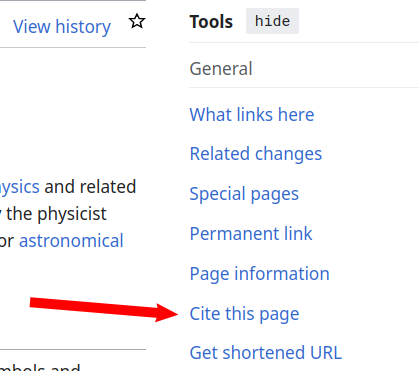
\includegraphics[width=\linewidth]{wikipedia-cite}
			\caption{Cite this page.}
			\label{fig:wiki-cite}
		\end{subfigure}
		%
		\hfill
		\begin{subfigure}[t]{0.65\textwidth}
			\centering
			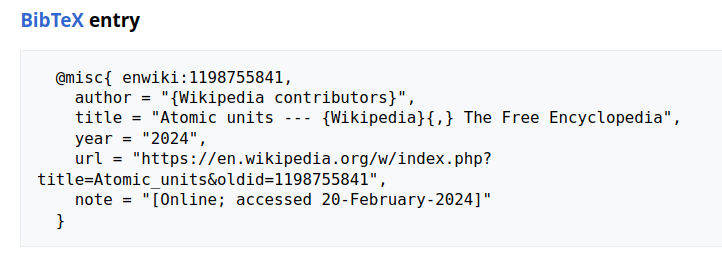
\includegraphics[width=\linewidth]{wikipedia-bibtex}
			\caption{Kod koji se kopira u \texttt{literatura.bib}.}
			\label{fig:wiki-bib}
		\end{subfigure}
		\caption{Citiranje s Wikipedije.}
	\end{figure}

	\begin{figure}[h]
		\centering
		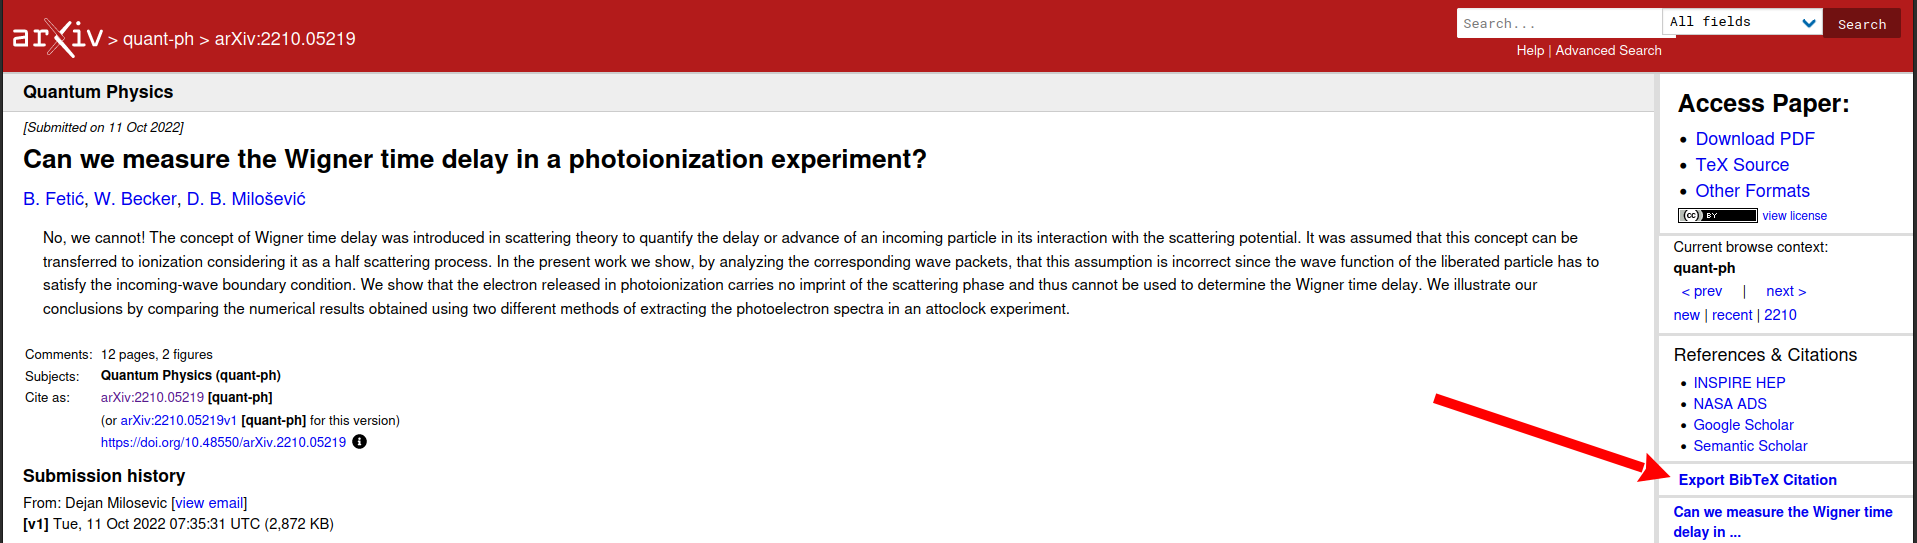
\includegraphics[width=\textwidth]{arxiv-cite}
		\caption{Citiranje s arXiva.}
		\label{fig:arxiv-cite}
	\end{figure}

	\paragraph{Napomena.}
	Ovo je \verb+\paragraph+, naslov koji se nastavlja u istom redu.
	Koristan je za kratke cjeline koje ne trebaju biti u sadržaju.

\section[Bespotrebno dug naslov]{Ovo je jako dug naslov koji kada bi ovako stajao u sadržaju bilo bi previše, dolazilo bi do preloma, i čitava stvari bi bila u 3 reda}
	Srećom, ako koristimo \verb+\section[Kratki naziv]{Puni naziv}+ to se ne
	dešava.
	Sličan pristup radi i sa slikama i tabelama,
	\verb+\caption[Kratki opis]{Detaljni opis}+, gdje je to puno teže izbjeći.


	% !TEX root = ../../main.tex
\chapter{Zaključak}
\label{ch:zakljucak}

Zaključak sažima glavne rezultate rada i odgovara na pitanja postavljena u
uvodu.
Ovdje je zgodno navesti i ograničenja korištenih metoda, kao i moguće pravce
daljeg istraživanja.


	%%%%%%%%%%%%%%%%%%%%%%%%%%%%%%%%%%%%%%%%%%%%%%%%%%%%%%%%%%%%%%%%%%%%%%%%%%%%%%%%%%%%%%%%%%

	\appendix

	% !TEX root = ../../main.tex
\chapter{Dodatak}
\label{ch:dodatak}

Poglavlja nakon \verb+\appendix+ u \texttt{main.tex} se numerišu slovima.
Ovdje idu dugački izvodi, dodatne tabele ili kod.

Vanjski PDF, npr.~nacrt, se umeće cijeli s
\begin{center}
	\verb+\includepdf[pages=-]{chapters/dodatak/nacrt.pdf}+
\end{center}
Za stranice okrenute na landscape dodati opcije \verb+landscape,angle=90+.


	%%%%%%%%%%%%%%%%%%%%%%%%%%%%%%%%%%%%%%%%%%%%%%%%%%%%%%%%%%%%%%%%%%%%%%%%%%%%%%%%%%%%%%%%%%

	\backmatter

	% Izbacuje sve izvore koji su u literatura.bib, i one koji nisu citirani.
	% \nocite{*}
	\printbibliography[title={Bibliografija},heading=bibintoc]

\end{document}
